% !TEX TS-program = pdflatex
% !TEX encoding = UTF-8 Unicode
\documentclass[border=0mm]{standalone}
% packages
\usepackage{tikz}
\usetikzlibrary{patterns}
\usepackage{amsmath,amssymb}
\usepackage{bm}
\usepackage{pgfplots}
\pgfplotsset{compat=1.15}
% start document
\begin{document}
% generated by ROOT (CERN)
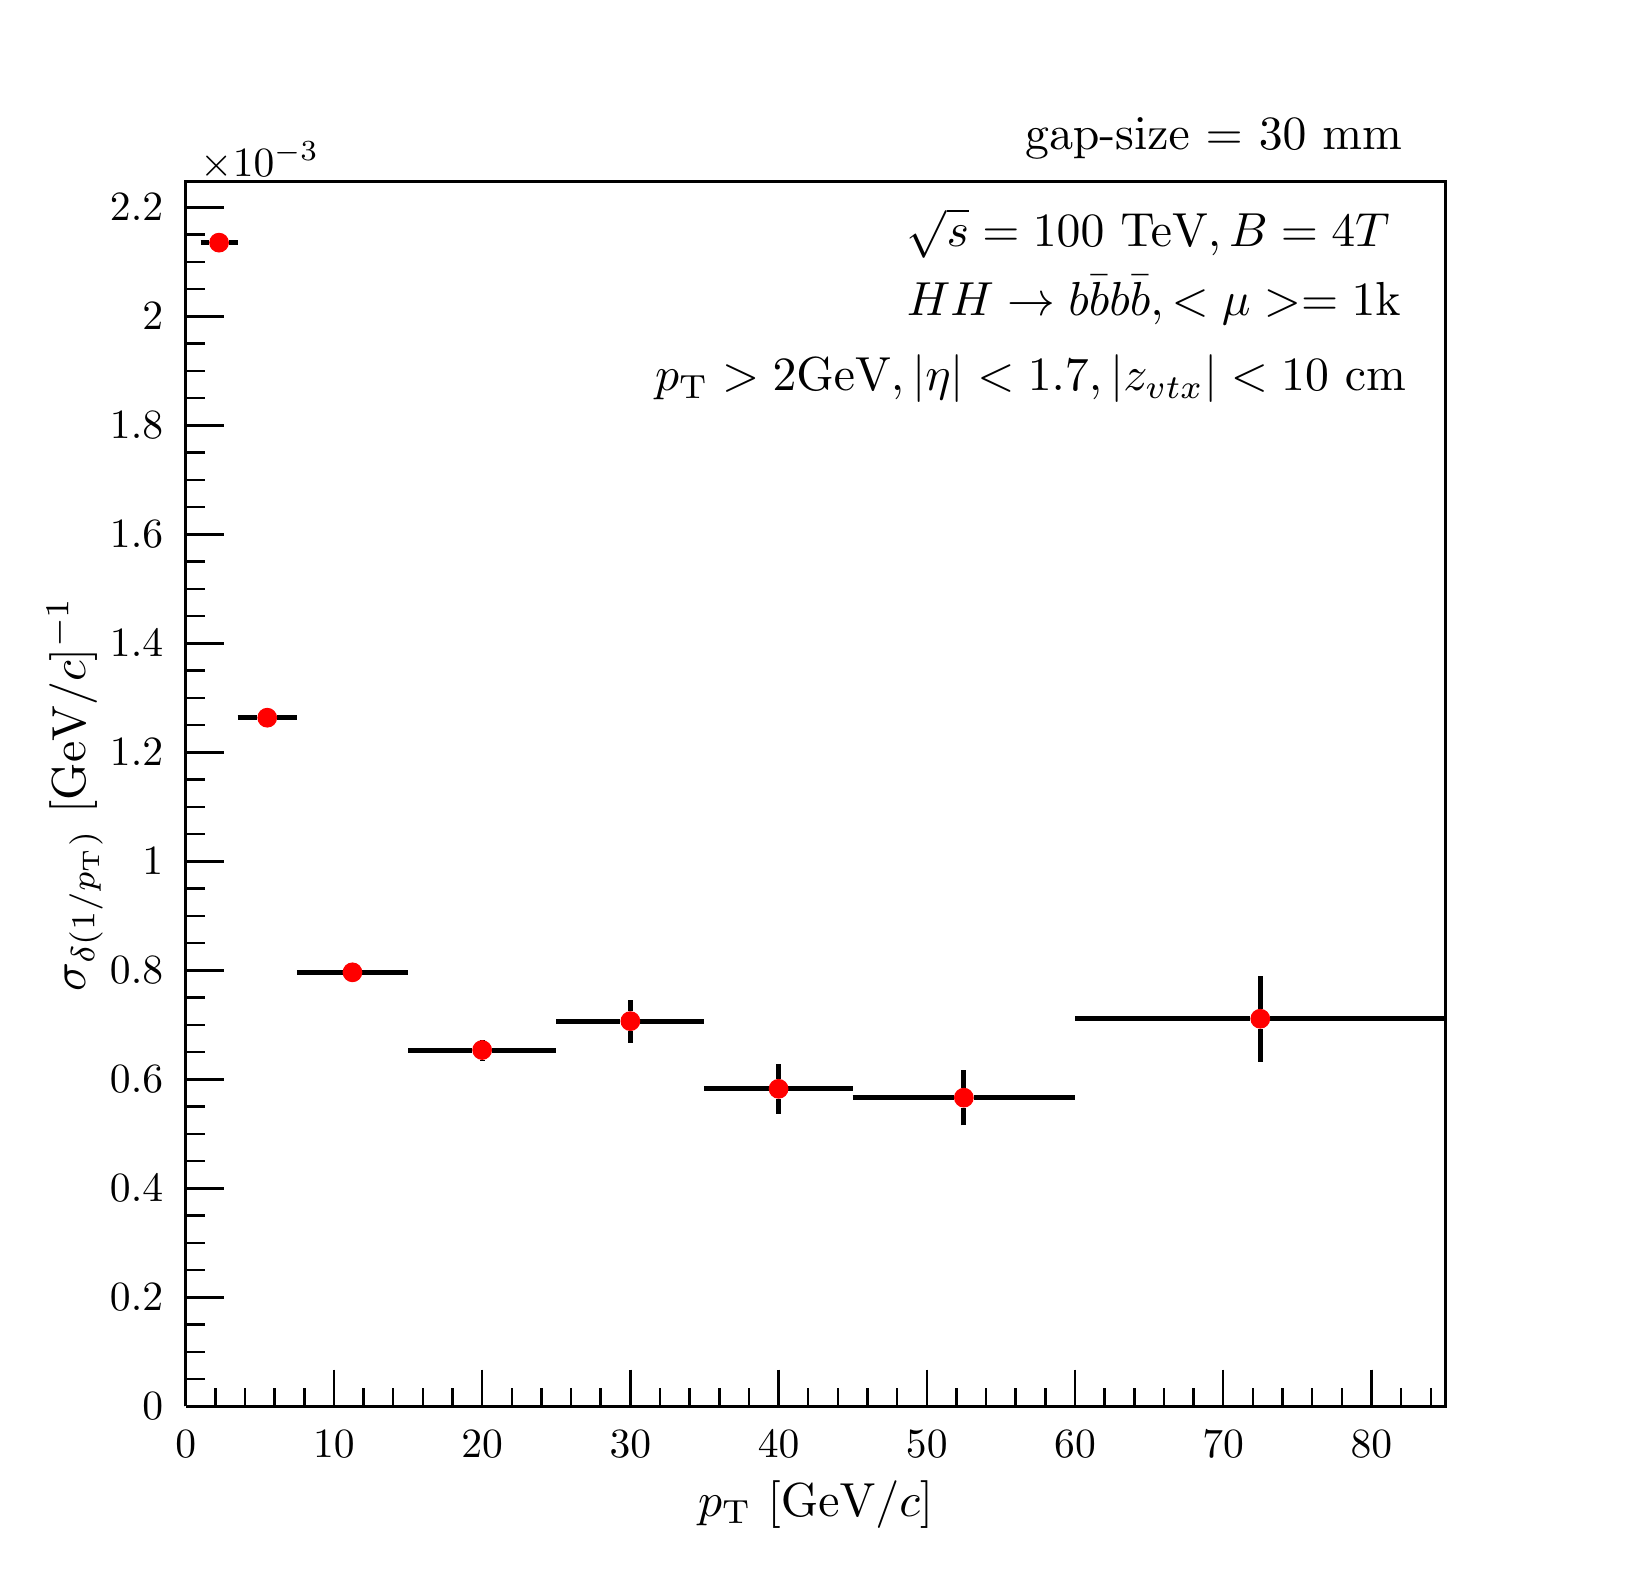
\begin{tikzpicture}
\pgfdeclareplotmark{cross} {
\pgfpathmoveto{\pgfpoint{-0.3\pgfplotmarksize}{\pgfplotmarksize}}
\pgfpathlineto{\pgfpoint{+0.3\pgfplotmarksize}{\pgfplotmarksize}}
\pgfpathlineto{\pgfpoint{+0.3\pgfplotmarksize}{0.3\pgfplotmarksize}}
\pgfpathlineto{\pgfpoint{+1\pgfplotmarksize}{0.3\pgfplotmarksize}}
\pgfpathlineto{\pgfpoint{+1\pgfplotmarksize}{-0.3\pgfplotmarksize}}
\pgfpathlineto{\pgfpoint{+0.3\pgfplotmarksize}{-0.3\pgfplotmarksize}}
\pgfpathlineto{\pgfpoint{+0.3\pgfplotmarksize}{-1.\pgfplotmarksize}}
\pgfpathlineto{\pgfpoint{-0.3\pgfplotmarksize}{-1.\pgfplotmarksize}}
\pgfpathlineto{\pgfpoint{-0.3\pgfplotmarksize}{-0.3\pgfplotmarksize}}
\pgfpathlineto{\pgfpoint{-1.\pgfplotmarksize}{-0.3\pgfplotmarksize}}
\pgfpathlineto{\pgfpoint{-1.\pgfplotmarksize}{0.3\pgfplotmarksize}}
\pgfpathlineto{\pgfpoint{-0.3\pgfplotmarksize}{0.3\pgfplotmarksize}}
\pgfpathclose
\pgfusepathqstroke
}
\pgfdeclareplotmark{cross*} {
\pgfpathmoveto{\pgfpoint{-0.3\pgfplotmarksize}{\pgfplotmarksize}}
\pgfpathlineto{\pgfpoint{+0.3\pgfplotmarksize}{\pgfplotmarksize}}
\pgfpathlineto{\pgfpoint{+0.3\pgfplotmarksize}{0.3\pgfplotmarksize}}
\pgfpathlineto{\pgfpoint{+1\pgfplotmarksize}{0.3\pgfplotmarksize}}
\pgfpathlineto{\pgfpoint{+1\pgfplotmarksize}{-0.3\pgfplotmarksize}}
\pgfpathlineto{\pgfpoint{+0.3\pgfplotmarksize}{-0.3\pgfplotmarksize}}
\pgfpathlineto{\pgfpoint{+0.3\pgfplotmarksize}{-1.\pgfplotmarksize}}
\pgfpathlineto{\pgfpoint{-0.3\pgfplotmarksize}{-1.\pgfplotmarksize}}
\pgfpathlineto{\pgfpoint{-0.3\pgfplotmarksize}{-0.3\pgfplotmarksize}}
\pgfpathlineto{\pgfpoint{-1.\pgfplotmarksize}{-0.3\pgfplotmarksize}}
\pgfpathlineto{\pgfpoint{-1.\pgfplotmarksize}{0.3\pgfplotmarksize}}
\pgfpathlineto{\pgfpoint{-0.3\pgfplotmarksize}{0.3\pgfplotmarksize}}
\pgfpathclose
\pgfusepathqfillstroke
}
\pgfdeclareplotmark{newstar} {
\pgfpathmoveto{\pgfqpoint{0pt}{\pgfplotmarksize}}
\pgfpathlineto{\pgfqpointpolar{44}{0.5\pgfplotmarksize}}
\pgfpathlineto{\pgfqpointpolar{18}{\pgfplotmarksize}}
\pgfpathlineto{\pgfqpointpolar{-20}{0.5\pgfplotmarksize}}
\pgfpathlineto{\pgfqpointpolar{-54}{\pgfplotmarksize}}
\pgfpathlineto{\pgfqpointpolar{-90}{0.5\pgfplotmarksize}}
\pgfpathlineto{\pgfqpointpolar{234}{\pgfplotmarksize}}
\pgfpathlineto{\pgfqpointpolar{198}{0.5\pgfplotmarksize}}
\pgfpathlineto{\pgfqpointpolar{162}{\pgfplotmarksize}}
\pgfpathlineto{\pgfqpointpolar{134}{0.5\pgfplotmarksize}}
\pgfpathclose
\pgfusepathqstroke
}
\pgfdeclareplotmark{newstar*} {
\pgfpathmoveto{\pgfqpoint{0pt}{\pgfplotmarksize}}
\pgfpathlineto{\pgfqpointpolar{44}{0.5\pgfplotmarksize}}
\pgfpathlineto{\pgfqpointpolar{18}{\pgfplotmarksize}}
\pgfpathlineto{\pgfqpointpolar{-20}{0.5\pgfplotmarksize}}
\pgfpathlineto{\pgfqpointpolar{-54}{\pgfplotmarksize}}
\pgfpathlineto{\pgfqpointpolar{-90}{0.5\pgfplotmarksize}}
\pgfpathlineto{\pgfqpointpolar{234}{\pgfplotmarksize}}
\pgfpathlineto{\pgfqpointpolar{198}{0.5\pgfplotmarksize}}
\pgfpathlineto{\pgfqpointpolar{162}{\pgfplotmarksize}}
\pgfpathlineto{\pgfqpointpolar{134}{0.5\pgfplotmarksize}}
\pgfpathclose
\pgfusepathqfillstroke
}
\definecolor{c}{rgb}{1,1,1};
\draw [color=c, fill=c] (0,0) rectangle (20,19.4486);
\draw [color=c, fill=c] (2,1.94486) rectangle (18,17.5038);
\definecolor{c}{rgb}{0,0,0};
\draw [c,line width=0.9] (2,1.94486) -- (2,17.5038) -- (18,17.5038) -- (18,1.94486) -- (2,1.94486);
\definecolor{c}{rgb}{1,1,1};
\draw [color=c, fill=c] (2,1.94486) rectangle (18,17.5038);
\definecolor{c}{rgb}{0,0,0};
\draw [c,line width=0.9] (2,1.94486) -- (2,17.5038) -- (18,17.5038) -- (18,1.94486) -- (2,1.94486);
\draw [c,line width=1.8] (2.18824,16.7253) -- (2.29822,16.7253);
\draw [c,line width=1.8] (2.54884,16.7253) -- (2.65882,16.7253);
\definecolor{c}{rgb}{1,0,0};
\foreach \P in {(2.42353,16.7253)}{\draw[mark options={color=c,fill=c},mark size=3.363363pt,mark=*] plot coordinates {\P};}
\definecolor{c}{rgb}{0,0,0};
\draw [c,line width=1.8] (2.65882,10.692) -- (2.90998,10.692);
\draw [c,line width=1.8] (3.16061,10.692) -- (3.41176,10.692);
\definecolor{c}{rgb}{1,0,0};
\foreach \P in {(3.03529,10.692)}{\draw[mark options={color=c,fill=c},mark size=3.363363pt,mark=*] plot coordinates {\P};}
\definecolor{c}{rgb}{0,0,0};
\draw [c,line width=1.8] (3.41176,7.45849) -- (3.99233,7.45849);
\draw [c,line width=1.8] (4.24296,7.45849) -- (4.82353,7.45849);
\definecolor{c}{rgb}{1,0,0};
\foreach \P in {(4.11765,7.45849)}{\draw[mark options={color=c,fill=c},mark size=3.363363pt,mark=*] plot coordinates {\P};}
\definecolor{c}{rgb}{0,0,0};
\draw [c,line width=1.8] (5.76471,6.34514) -- (5.76471,6.34649);
\draw [c,line width=1.8] (5.76471,6.59712) -- (5.76471,6.59847);
\draw [c,line width=1.8] (4.82353,6.4718) -- (5.63939,6.4718);
\draw [c,line width=1.8] (5.89002,6.4718) -- (6.70588,6.4718);
\definecolor{c}{rgb}{1,0,0};
\foreach \P in {(5.76471,6.4718)}{\draw[mark options={color=c,fill=c},mark size=3.363363pt,mark=*] plot coordinates {\P};}
\definecolor{c}{rgb}{0,0,0};
\draw [c,line width=1.8] (7.64706,6.56675) -- (7.64706,6.71354);
\draw [c,line width=1.8] (7.64706,6.96417) -- (7.64706,7.11095);
\draw [c,line width=1.8] (6.70588,6.83885) -- (7.52175,6.83885);
\draw [c,line width=1.8] (7.77237,6.83885) -- (8.58823,6.83885);
\definecolor{c}{rgb}{1,0,0};
\foreach \P in {(7.64706,6.83885)}{\draw[mark options={color=c,fill=c},mark size=3.363363pt,mark=*] plot coordinates {\P};}
\definecolor{c}{rgb}{0,0,0};
\draw [c,line width=1.8] (9.52941,5.66269) -- (9.52941,5.85361);
\draw [c,line width=1.8] (9.52941,6.10424) -- (9.52941,6.29515);
\draw [c,line width=1.8] (8.58823,5.97892) -- (9.4041,5.97892);
\draw [c,line width=1.8] (9.65473,5.97892) -- (10.4706,5.97892);
\definecolor{c}{rgb}{1,0,0};
\foreach \P in {(9.52941,5.97892)}{\draw[mark options={color=c,fill=c},mark size=3.363363pt,mark=*] plot coordinates {\P};}
\definecolor{c}{rgb}{0,0,0};
\draw [c,line width=1.8] (11.8824,5.51461) -- (11.8824,5.74117);
\draw [c,line width=1.8] (11.8824,5.99179) -- (11.8824,6.21835);
\draw [c,line width=1.8] (10.4706,5.86648) -- (11.757,5.86648);
\draw [c,line width=1.8] (12.0077,5.86648) -- (13.2941,5.86648);
\definecolor{c}{rgb}{1,0,0};
\foreach \P in {(11.8824,5.86648)}{\draw[mark options={color=c,fill=c},mark size=3.363363pt,mark=*] plot coordinates {\P};}
\definecolor{c}{rgb}{0,0,0};
\draw [c,line width=1.8] (15.6471,6.3201) -- (15.6471,6.7436);
\draw [c,line width=1.8] (15.6471,6.99423) -- (15.6471,7.41773);
\draw [c,line width=1.8] (13.2941,6.86892) -- (15.5217,6.86892);
\draw [c,line width=1.8] (15.7724,6.86892) -- (18,6.86892);
\definecolor{c}{rgb}{1,0,0};
\foreach \P in {(15.6471,6.86892)}{\draw[mark options={color=c,fill=c},mark size=3.363363pt,mark=*] plot coordinates {\P};}
\definecolor{c}{rgb}{0,0,0};
\draw [c,line width=0.9] (2,1.94486) -- (18,1.94486);
\draw [c,line width=0.9] (2,2.41163) -- (2,1.94486);
\draw [c,line width=0.9] (2.37647,2.17825) -- (2.37647,1.94486);
\draw [c,line width=0.9] (2.75294,2.17825) -- (2.75294,1.94486);
\draw [c,line width=0.9] (3.12941,2.17825) -- (3.12941,1.94486);
\draw [c,line width=0.9] (3.50588,2.17825) -- (3.50588,1.94486);
\draw [c,line width=0.9] (3.88235,2.41163) -- (3.88235,1.94486);
\draw [c,line width=0.9] (4.25882,2.17825) -- (4.25882,1.94486);
\draw [c,line width=0.9] (4.63529,2.17825) -- (4.63529,1.94486);
\draw [c,line width=0.9] (5.01177,2.17825) -- (5.01177,1.94486);
\draw [c,line width=0.9] (5.38824,2.17825) -- (5.38824,1.94486);
\draw [c,line width=0.9] (5.76471,2.41163) -- (5.76471,1.94486);
\draw [c,line width=0.9] (6.14118,2.17825) -- (6.14118,1.94486);
\draw [c,line width=0.9] (6.51765,2.17825) -- (6.51765,1.94486);
\draw [c,line width=0.9] (6.89412,2.17825) -- (6.89412,1.94486);
\draw [c,line width=0.9] (7.27059,2.17825) -- (7.27059,1.94486);
\draw [c,line width=0.9] (7.64706,2.41163) -- (7.64706,1.94486);
\draw [c,line width=0.9] (8.02353,2.17825) -- (8.02353,1.94486);
\draw [c,line width=0.9] (8.4,2.17825) -- (8.4,1.94486);
\draw [c,line width=0.9] (8.77647,2.17825) -- (8.77647,1.94486);
\draw [c,line width=0.9] (9.15294,2.17825) -- (9.15294,1.94486);
\draw [c,line width=0.9] (9.52941,2.41163) -- (9.52941,1.94486);
\draw [c,line width=0.9] (9.90588,2.17825) -- (9.90588,1.94486);
\draw [c,line width=0.9] (10.2824,2.17825) -- (10.2824,1.94486);
\draw [c,line width=0.9] (10.6588,2.17825) -- (10.6588,1.94486);
\draw [c,line width=0.9] (11.0353,2.17825) -- (11.0353,1.94486);
\draw [c,line width=0.9] (11.4118,2.41163) -- (11.4118,1.94486);
\draw [c,line width=0.9] (11.7882,2.17825) -- (11.7882,1.94486);
\draw [c,line width=0.9] (12.1647,2.17825) -- (12.1647,1.94486);
\draw [c,line width=0.9] (12.5412,2.17825) -- (12.5412,1.94486);
\draw [c,line width=0.9] (12.9176,2.17825) -- (12.9176,1.94486);
\draw [c,line width=0.9] (13.2941,2.41163) -- (13.2941,1.94486);
\draw [c,line width=0.9] (13.6706,2.17825) -- (13.6706,1.94486);
\draw [c,line width=0.9] (14.0471,2.17825) -- (14.0471,1.94486);
\draw [c,line width=0.9] (14.4235,2.17825) -- (14.4235,1.94486);
\draw [c,line width=0.9] (14.8,2.17825) -- (14.8,1.94486);
\draw [c,line width=0.9] (15.1765,2.41163) -- (15.1765,1.94486);
\draw [c,line width=0.9] (15.5529,2.17825) -- (15.5529,1.94486);
\draw [c,line width=0.9] (15.9294,2.17825) -- (15.9294,1.94486);
\draw [c,line width=0.9] (16.3059,2.17825) -- (16.3059,1.94486);
\draw [c,line width=0.9] (16.6824,2.17825) -- (16.6824,1.94486);
\draw [c,line width=0.9] (17.0588,2.41163) -- (17.0588,1.94486);
\draw [c,line width=0.9] (17.0588,2.41163) -- (17.0588,1.94486);
\draw [c,line width=0.9] (17.4353,2.17825) -- (17.4353,1.94486);
\draw [c,line width=0.9] (17.8118,2.17825) -- (17.8118,1.94486);
\draw [anchor=base] (2,1.30306) node[scale=1.50291, color=c, rotate=0]{0};
\draw [anchor=base] (3.88235,1.30306) node[scale=1.50291, color=c, rotate=0]{10};
\draw [anchor=base] (5.76471,1.30306) node[scale=1.50291, color=c, rotate=0]{20};
\draw [anchor=base] (7.64706,1.30306) node[scale=1.50291, color=c, rotate=0]{30};
\draw [anchor=base] (9.52941,1.30306) node[scale=1.50291, color=c, rotate=0]{40};
\draw [anchor=base] (11.4118,1.30306) node[scale=1.50291, color=c, rotate=0]{50};
\draw [anchor=base] (13.2941,1.30306) node[scale=1.50291, color=c, rotate=0]{60};
\draw [anchor=base] (15.1765,1.30306) node[scale=1.50291, color=c, rotate=0]{70};
\draw [anchor=base] (17.0588,1.30306) node[scale=1.50291, color=c, rotate=0]{80};
\draw (10,0.700151) node[scale=1.72557, color=c, rotate=0]{$p_{\text{T}} ~[\text{GeV}/c]$};
\draw [c,line width=0.9] (2,1.94486) -- (2,17.5038);
\draw [c,line width=0.9] (2.48,1.94486) -- (2,1.94486);
\draw [c,line width=0.9] (2.24,2.29093) -- (2,2.29093);
\draw [c,line width=0.9] (2.24,2.637) -- (2,2.637);
\draw [c,line width=0.9] (2.24,2.98307) -- (2,2.98307);
\draw [c,line width=0.9] (2.48,3.32914) -- (2,3.32914);
\draw [c,line width=0.9] (2.24,3.6752) -- (2,3.6752);
\draw [c,line width=0.9] (2.24,4.02127) -- (2,4.02127);
\draw [c,line width=0.9] (2.24,4.36734) -- (2,4.36734);
\draw [c,line width=0.9] (2.48,4.71341) -- (2,4.71341);
\draw [c,line width=0.9] (2.24,5.05948) -- (2,5.05948);
\draw [c,line width=0.9] (2.24,5.40554) -- (2,5.40554);
\draw [c,line width=0.9] (2.24,5.75161) -- (2,5.75161);
\draw [c,line width=0.9] (2.48,6.09768) -- (2,6.09768);
\draw [c,line width=0.9] (2.24,6.44375) -- (2,6.44375);
\draw [c,line width=0.9] (2.24,6.78982) -- (2,6.78982);
\draw [c,line width=0.9] (2.24,7.13589) -- (2,7.13589);
\draw [c,line width=0.9] (2.48,7.48195) -- (2,7.48195);
\draw [c,line width=0.9] (2.24,7.82802) -- (2,7.82802);
\draw [c,line width=0.9] (2.24,8.17409) -- (2,8.17409);
\draw [c,line width=0.9] (2.24,8.52016) -- (2,8.52016);
\draw [c,line width=0.9] (2.48,8.86623) -- (2,8.86623);
\draw [c,line width=0.9] (2.24,9.2123) -- (2,9.2123);
\draw [c,line width=0.9] (2.24,9.55836) -- (2,9.55836);
\draw [c,line width=0.9] (2.24,9.90443) -- (2,9.90443);
\draw [c,line width=0.9] (2.48,10.2505) -- (2,10.2505);
\draw [c,line width=0.9] (2.24,10.5966) -- (2,10.5966);
\draw [c,line width=0.9] (2.24,10.9426) -- (2,10.9426);
\draw [c,line width=0.9] (2.24,11.2887) -- (2,11.2887);
\draw [c,line width=0.9] (2.48,11.6348) -- (2,11.6348);
\draw [c,line width=0.9] (2.24,11.9808) -- (2,11.9808);
\draw [c,line width=0.9] (2.24,12.3269) -- (2,12.3269);
\draw [c,line width=0.9] (2.24,12.673) -- (2,12.673);
\draw [c,line width=0.9] (2.48,13.019) -- (2,13.019);
\draw [c,line width=0.9] (2.24,13.3651) -- (2,13.3651);
\draw [c,line width=0.9] (2.24,13.7112) -- (2,13.7112);
\draw [c,line width=0.9] (2.24,14.0573) -- (2,14.0573);
\draw [c,line width=0.9] (2.48,14.4033) -- (2,14.4033);
\draw [c,line width=0.9] (2.24,14.7494) -- (2,14.7494);
\draw [c,line width=0.9] (2.24,15.0955) -- (2,15.0955);
\draw [c,line width=0.9] (2.24,15.4415) -- (2,15.4415);
\draw [c,line width=0.9] (2.48,15.7876) -- (2,15.7876);
\draw [c,line width=0.9] (2.24,16.1337) -- (2,16.1337);
\draw [c,line width=0.9] (2.24,16.4797) -- (2,16.4797);
\draw [c,line width=0.9] (2.24,16.8258) -- (2,16.8258);
\draw [c,line width=0.9] (2.48,17.1719) -- (2,17.1719);
\draw [c,line width=0.9] (2.48,17.1719) -- (2,17.1719);
\draw [anchor= east] (1.9,1.94486) node[scale=1.50291, color=c, rotate=0]{0};
\draw [anchor= east] (1.9,3.32914) node[scale=1.50291, color=c, rotate=0]{0.2};
\draw [anchor= east] (1.9,4.71341) node[scale=1.50291, color=c, rotate=0]{0.4};
\draw [anchor= east] (1.9,6.09768) node[scale=1.50291, color=c, rotate=0]{0.6};
\draw [anchor= east] (1.9,7.48195) node[scale=1.50291, color=c, rotate=0]{0.8};
\draw [anchor= east] (1.9,8.86623) node[scale=1.50291, color=c, rotate=0]{1};
\draw [anchor= east] (1.9,10.2505) node[scale=1.50291, color=c, rotate=0]{1.2};
\draw [anchor= east] (1.9,11.6348) node[scale=1.50291, color=c, rotate=0]{1.4};
\draw [anchor= east] (1.9,13.019) node[scale=1.50291, color=c, rotate=0]{1.6};
\draw [anchor= east] (1.9,14.4033) node[scale=1.50291, color=c, rotate=0]{1.8};
\draw [anchor= east] (1.9,15.7876) node[scale=1.50291, color=c, rotate=0]{2};
\draw [anchor= east] (1.9,17.1719) node[scale=1.50291, color=c, rotate=0]{2.2};
\draw [anchor=base west] (2,17.5718) node[scale=1.50291, color=c, rotate=0]{$\times10^{-3}$};
\draw (0.592,9.72431) node[scale=1.72557, color=c, rotate=90]{$\sigma_{\delta(1/p_{\text{T}})} ~[\text{GeV}/c]^{-1}$};
\draw [anchor=base west] (10.945,16.6748) node[scale=1.72557, color=c, rotate=0]{$\sqrt{s} = 100 ~\text{TeV}, B = 4T$};
\draw [anchor=base west] (10.945,15.7996) node[scale=1.72557, color=c, rotate=0]{$HH \rightarrow b\bar{b}b\bar{b}, <\mu> = \text{1k}$};
\draw [anchor=base east] (17.7105,14.8432) node[scale=1.72557, color=c, rotate=0]{$p_{\text{T}} > 2\text{GeV}, |\eta| < 1.7, |z_{vtx}| < 10\text{~cm}$};
\draw [anchor=base west] (12.445,17.9122) node[scale=1.72557, color=c, rotate=0]{gap-size = 30 mm};
\draw [anchor=base west] (12.445,17.5232) node[scale=1.72557, color=c, rotate=0]{ };
\end{tikzpicture}
% end document
\end{document}
